\documentclass{beamer}
\usepackage{amsmath}
\usepackage[english]{babel} %set language; note: after changing this, you need to delete all auxiliary files to recompile
\usepackage[utf8]{inputenc} %define file encoding; latin1 is the other often used option
\usepackage{csquotes} % provides context sensitive quotation facilities
\usepackage{graphicx} %allows for inserting figures
\usepackage{booktabs} % for table formatting without vertical lines
\usepackage{textcomp} % allow for example using the Euro sign with \texteuro
\usepackage{stackengine}
\usepackage{wasysym}
\usepackage{tikzsymbols}
\usepackage{textcomp}
\usepackage{xcolor}
\usepackage[dvipsnames]{xcolor}
\usepackage{colortbl}
\usepackage{adjustbox}
\newcommand{\bubblethis}[2]{
        \tikz[remember picture,baseline]{\node[anchor=base,inner sep=0,outer sep=0]%
        (#1) {\underline{#1}};\node[overlay,cloud callout,callout relative pointer={(0.2cm,-0.7cm)},%
        aspect=2.5,fill=yellow!90] at ($(#1.north)+(-0.5cm,1.6cm)$) {#2};}%
    }%
\tikzset{face/.style={shape=circle,minimum size=4ex,shading=radial,outer sep=0pt,
        inner color=white!50!yellow,outer color= yellow!70!orange}}
%% Some commands to make the code easier
\newcommand{\emoticon}[1][]{%
  \node[face,#1] (emoticon) {};
  %% The eyes are fixed.
  \draw[fill=white] (-1ex,0ex) ..controls (-0.5ex,0.2ex)and(0.5ex,0.2ex)..
        (1ex,0.0ex) ..controls ( 1.5ex,1.5ex)and( 0.2ex,1.7ex)..
        (0ex,0.4ex) ..controls (-0.2ex,1.7ex)and(-1.5ex,1.5ex)..
        (-1ex,0ex)--cycle;}
\newcommand{\pupils}{
  %% standard pupils
  \fill[shift={(0.5ex,0.5ex)},rotate=80] 
       (0,0) ellipse (0.3ex and 0.15ex);
  \fill[shift={(-0.5ex,0.5ex)},rotate=100] 
       (0,0) ellipse (0.3ex and 0.15ex);}

\newcommand{\emoticonname}[1]{
  \node[below=1ex of emoticon,font=\footnotesize,
        minimum width=4cm]{#1};}
\usepackage{scalerel}
\usetikzlibrary{positioning}
\usepackage{xcolor,amssymb}
\newcommand\dangersignb[1][2ex]{%
  \scaleto{\stackengine{0.3pt}{\scalebox{1.1}[.9]{%
  \color{red}$\blacktriangle$}}{\tiny\bfseries !}{O}{c}{F}{F}{L}}{#1}%
}
\newcommand\dangersignw[1][2ex]{%
  \scaleto{\stackengine{0.3pt}{\scalebox{1.1}[.9]{%
  \color{red}$\blacktriangle$}}{\color{white}\tiny\bfseries !}{O}{c}{F}{F}{L}}{#1}%
}
\usepackage{fontawesome} % Social Icons
\usepackage{epstopdf} % allow embedding eps-figures
\usepackage{tikz} % allows drawing figures
\usepackage{amsmath,amssymb,amsthm} %advanced math facilities
\usepackage{lmodern} %uses font that support italic and bold at the same time
\usepackage{hyperref}
\usepackage{tikz}
\usepackage{tcolorbox}


\usefonttheme[onlymath]{serif} %set math font to serif ones

\definecolor{beamerblue}{rgb}{0.2,0.2,0.7} %define beamerblue color for later use

%%% defines highlight command to set text blue
\newcommand{\highlight}[1]{{\color{blue}{#1}}}


%%%%%%% commands defining backup slides so that frame numbering is correct

\newcommand{\backupbegin}{
   \newcounter{framenumberappendix}
   \setcounter{framenumberappendix}{\value{framenumber}}
}
\newcommand{\backupend}{
   \addtocounter{framenumberappendix}{-\value{framenumber}}
   \addtocounter{framenumber}{\value{framenumberappendix}}
}

%%%% end of defining backup slides

%Specify figure caption, see also http://tex.stackexchange.com/questions/155738/caption-package-not-working-with-beamer
\setbeamertemplate{caption}{\insertcaption} %redefines caption to remove label "Figure".
%\setbeamerfont{caption}{size=\scriptsize,shape=\itshape,series=\bfseries} %sets figure  caption bold and italic and makes it smaller

\newtcolorbox{boxA}{
    fontupper = \bf,
    boxrule = 1.5pt,
    colframe = black % frame color
}
\newtcolorbox{boxB}{
    boxrule = 1.5pt,
    colframe = blue!70!black,, % frame color
    colback = blue!7!white,
}



\usetheme{Boadilla}

% --------------------
% Overall information
% --------------------
\title[Economía I]{Economía I \vspace{4mm}
\\ Magistral 20: El Mecano}
\date{}
\author[Franco Riottini]{Franco Riottini}
\vspace{0.4cm}
\institute[]{Universidad de San Andrés}


\begin{document}

\begin{frame}
\titlepage
\centering

\includegraphics[scale=0.2]{../Figures/logoUDESA.jpg} 
\end{frame}

\begin{frame}{El mecano de la economía}
    \begin{itemize}
        \item Denominaremos \textbf{mecano de la economía} al funcionamiento articulado de \textbf{cuatro mercados}:
        \begin{itemize}
            \item Mercado de trabajo
            \item Mercado de bienes y servicios
            \item Mercado de dinero 
            \item Mercado de crédito    
        \end{itemize}
        \vspace{2mm}
        \item La interacción de estos cuatro grandes mercados determinará el equilibrio de las \textbf{variables macroeconómicas}:
        \begin{itemize}
            \item PBI de la economía
            \item Tasa de interés
            \item Nivel general de precios (e inflación)
            \item Salarios  
            \item Nivel de empleo
        \end{itemize}
        \begin{boxB}
            \centering
            Estaremos siempre pensando en una \textbf{economía cerrada}, es decir, \textit{sin comercio internacional}. 
        \end{boxB} 
    \end{itemize}
\end{frame}

\begin{frame}{El mercado de bienes y servicios}
\begin{itemize}
    \item \textcolor{blue!80!black}{\textbf{Demanda Agregada}}     {\textcolor{blue!80!black}{\faCartPlus}} \\ \vspace{1mm}
    \begin{itemize}
    \item Es la voluntad de gasto o el gasto planificado por los agentes en bienes y servicios finales dado un nivel de precios.
    \item ``Lo que estamos dispuestos a comprar". 
            \begin{center}
            \begin{tcolorbox}[width=3in, boxsep=0pt, left=0pt, right=0pt, top=2pt, ,colframe = blue!70!black, colback = blue!7!white]%%
                    $$ DA = C + I + G $$
             \end{tcolorbox}
             \end{center}
    \end{itemize} \vspace{2mm}
    \item \textcolor{blue!80!black}{\textbf{Oferta Agregada}}     {\textcolor{blue!80!black}{\faCogs}} \vspace{1mm}
    \begin{itemize}
    \item Es la capacidad productiva de la economía, en otras palabras, el PBI real. \vspace{1mm}
    \item ``Lo que podemos producir con los recursos y tecnología". 
        \begin{center}
            \begin{tcolorbox}[width=2in, boxsep=0pt, left=0pt, right=0pt, top=2pt, ,colframe = blue!70!black, colback = blue!7!white]%%
                    $$ OA = Y =f(K,L)$$
            \end{tcolorbox}
        \end{center}
    \end{itemize}
\end{itemize}

\vspace{2mm}
\begin{itemize}
    \item ¿Que forma tiene la oferta agregada y como se determina?
    \begin{itemize}
    \item Depende del enfoque que adoptemos: clásicos o keynesianos.
    \end{itemize}
\end{itemize}
\end{frame}

\begin{frame}{El mercado de trabajo}
\begin{itemize}
    \item El mercado de trabajo determina el empleo, desempleo y salarios. \vspace{1mm}
    \item La \textbf{demanda de trabajo} representa a todas las empresas, gobiernos u organizaciones que desean contratar empleados u horas de trabajo. 
            \begin{center}
            \begin{tcolorbox}[width=3.5in,boxsep=0pt, left=0pt, right=0pt, top=0pt,colframe = blue!70!black, colback = blue!7!white]%%
             $$ \text{Demanda de trabajo}= T_d (W, P, PMgT)$$
             \end{tcolorbox}
             \end{center}
             \vspace{1mm} 
    \item La \textbf{oferta de trabajo} está compuesta por todas las personas que buscan trabajar. 
         \begin{center}
            \begin{tcolorbox}[width=3in, boxsep=0pt, left=0pt, right=0pt, top=2pt, ,colframe = blue!70!black, colback = blue!7!white]%%
              $$\text{Oferta de trabajo}= T_o (W)$$
             \end{tcolorbox}
             \end{center}
    \item ¿Cómo funciona este mercado?
    \begin{itemize}
        \item Los ``clásicos" consideran que opera de forma eficiente, es decir, las personas que desean trabajar terminan encontrando empleo.
        \item Los ``keynesianos" argumentan que presenta importantes deficiencias (rigidez nominal del salario), dando lugar al desempleo involuntario.
    \end{itemize}
\end{itemize}
\end{frame}


\begin{frame}{El mercado de dinero}
\begin{itemize}
    \item En el mercado de dinero se intercambia  poder de compra, es decir, dinero.
    \item \textbf{Demanda de Dinero}: cuánto dinero desea tener la sociedad. 
            \begin{center}
            \begin{tcolorbox}[width=2in, boxsep=0pt, left=0pt, right=0pt, top=2pt,colframe = blue!70!black, colback = blue!7!white]%%
                    $$ M_{d}=f(Y, i, P) $$
             \end{tcolorbox}
             \end{center} 
     \item \textbf{Oferta de Dinero}: cuánto emite el Banco Central y el efecto del multiplicador monetario.
     \item El mercado de dinero se equilibra cuando:
     \begin{center}
            \begin{tcolorbox}[width=2.5in, boxsep=0pt, left=0pt, right=0pt, top=2pt,colframe = blue!70!black, colback = blue!7!white]%%
                    $$Ms= M_{d}=f(Y, i, P) $$
             \end{tcolorbox}
    \end{center} 
    \item Según en que enfoque nos ubiquemos, el equilibrio se va a dar en un punto distinto:
    \begin{itemize}
        \item Corto plazo keynesiano: determina la tasa de interés.
        \item Largo plazo clásico: determina la cantidad de dinero $\rightarrow$ lo cual determina el nivel de precios.
    \end{itemize}
\end{itemize}
\end{frame}

\begin{frame}{El mercado de crédito}
    \begin{itemize}
        \item Este mercado conecta a quienes desean postergar consumo hoy para ahorrar, con quienes necesitan recursos para invertir y producir.
        \item \textbf{Demanda de Crédito}: Deuda pública e Inversión.
        \item \textbf{Oferta de Crédito}: Ahorro interno.
        \item El equilibrio se alcanza cuando el volumen total de inversión deseada coincide con el ahorro disponible en la economía:
                \begin{center}
                \begin{tcolorbox}[width=2in, boxsep=0pt, left=0pt, right=0pt, top=2pt,colframe = blue!70!black, colback = blue!7!white]%%
                        $$ I(i,Y)=A(i,Y) $$
                \end{tcolorbox}
                \end{center}
        \item Este mercado también va verse distinto depende del enfoque que adoptemos:
        \begin{itemize}
            \item Corto plazo keynesiano: afecta más al nivel de producto.
            \item Largo plazo clásico: afecta más a la tasa de interés.
        \end{itemize}
    \end{itemize}
\end{frame}

\begin{frame}{El enfoque clásico y keynesiano}

    \begin{itemize}
        \item Según la \textcolor{green}{visión que se tenga del mercado de trabajo}, el producto se va a determinar por la oferta o por la demanda agregada. 
        \item Para los \textbf{Clásicos} es la capacidad productiva \faCogs:
            \begin{center}
            \begin{tcolorbox}[width=2in, boxsep=0pt, left=0pt, right=0pt, top=2pt, ,colframe = blue!70!black, colback = blue!7!white ]%%
                    $$ \bar{Y}=f(K, L) $$
             \end{tcolorbox}
             \end{center}
             
            \begin{itemize}
            \item \textcolor{green}{Los factores de producción están plenamente ocupados}
            \item Se produce el PBI ``potencial"
              \item ``Ley de Say" (la oferta encuentra su demanda)
            \end{itemize}
            
        \vspace{2mm}
        \item Para los \textbf{Keynesianos} es la demanda \faCartPlus:
            
            \begin{center}
            \begin{tcolorbox}[width=2in, boxsep=0pt, left=0pt, right=0pt, top=2pt, ,colframe = blue!70!black, colback = blue!7!white]%%
                    $$ Y = C + I + G  \leq \bar{Y} $$
             \end{tcolorbox}
             \end{center}
             
            \begin{itemize}
            \item  \textcolor{green}{En el mercado de trabajo, los salarios son ``rígidos a la baja"}
            \item La demanda se ubica por debajo de la capacidad productiva. 
            \item Entonces el producto lo define la demanda agregada.
            \end{itemize}
    \end{itemize}

\end{frame}

\begin{frame}{El enfoque clásico y keynesiano: oferta agregada}

    \begin{itemize}
            \item La curva OA relaciona P (precios) con Y (producto).
    \end{itemize}
    \begin{center}
    \begin{figure}[H]
    \renewcommand{\figurename}{Figure}
    \begin{center}
        \begin{minipage}[b]{0.49\textwidth}
        \begin{center}
        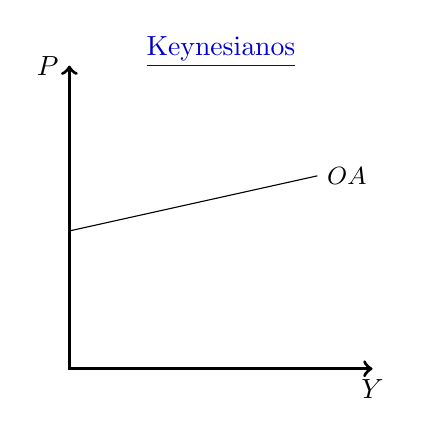
\begin{tikzpicture}[scale=0.35]
        \draw[very thick,<->] (0,11) node[left]{$P$}--(0,0)--(11,0) node[below]{$Y$};
        \draw[thin](0,5)--(9,7) node [right] {\small $OA$};
        \node[] at(5.5,11.5) {\textcolor{blue!80!black}{\underline{Keynesianos}}};
        \end{tikzpicture}
        \end{center}
        \begin{itemize}
        \footnotesize{
            \item Los precios son rígidos o se ajustan lentamente. Como hay recursos ociosos, se producirá más si la demanda lo requiere.
        }
        \end{itemize}
        
        \end{minipage}
      %  \hfill
        \begin{minipage}[b]{0.47\textwidth}
        \begin{center}
        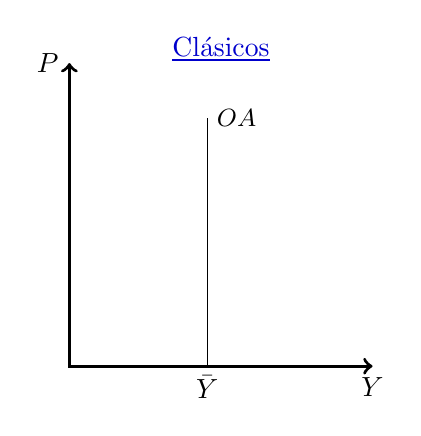
\begin{tikzpicture}[scale=0.35]
        \draw[very thick,<->] (0,11) node[left]{$P$}--(0,0)--(11,0) node[below]{$Y$};
        \draw[thin](5,0)--(5,9) node [right] {\small $OA$};
        \node[] at(5.5,11.5) {\textcolor{blue!80!black}{\underline{Clásicos}}};
        \node[below] at(5,0) {$\bar{Y}$};
        \end{tikzpicture}
        \end{center}
        \begin{itemize}
        \footnotesize{
            \item El producto está determinado por la capacidad productiva (pleno empleo), independientemente del nivel de precios. 
        }
        \end{itemize}
        \end{minipage}
    \end{center}
    \end{figure}
    \end{center} 

\end{frame}


\begin{frame}{El enfoque clásico y keynesiano: demanda agregada}
    \begin{itemize}
    \item La demanda luce similar en el mundo clásico y keynesiano.
    \item Relaciona al $C$ (consumo), $I$ (inversión) y $G$ (gasto) con el nivel de $P$ (precios). 
    \end{itemize}
\vspace{-5mm}
\begin{center}
    \begin{figure}[H]
    \begin{center}
    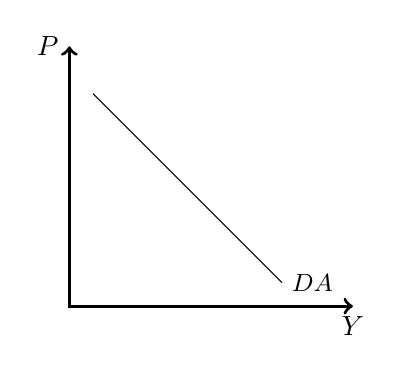
\begin{tikzpicture}[scale=0.3]
    \draw[very thick,<->] (0,11) node[left]{$P$}--(0,0)--(12,0) node[below]{$Y$};
    \draw[thin](1,9)--(9,1) node [right] {\small$DA$};
    \end{tikzpicture}
    \end{center}
    \end{figure}
\end{center}
\vspace{-3mm}
    \begin{itemize}
    \item Hay dos canales que explica la relación negativa entre $DA$ y $P$:
        \begin{itemize}
            \item Efecto riqueza: cuando suben los precios, el dinero vale menos. 
            \item Efecto tasa de interés: un aumento de $P$ sin cambiar $M$ lleva a tasas de interés más altas que hacen caer $C$ e $I$.
        \end{itemize}
    \end{itemize}

\end{frame}



\begin{frame}{Shocks a la Demanda Agregada}

\begin{columns}
  \column{0.5\textwidth} 
    \begin{center}
    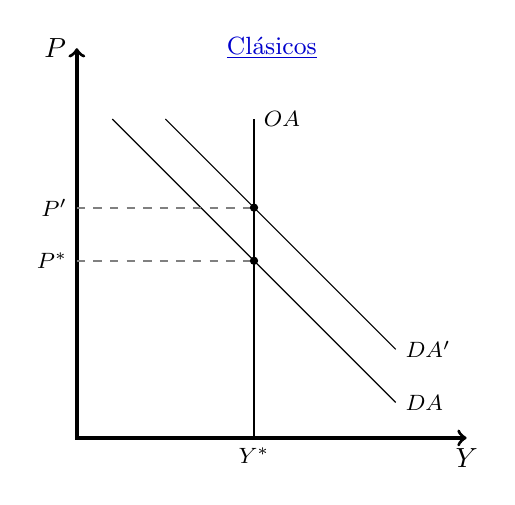
\begin{tikzpicture}[scale=0.45]
    \draw[very thick,<->] (0,11) node[left]{$P$}--(0,0)--(11,0) node[below]{$Y$};
    \draw[thin](5,0)--(5,9) node [right] {\footnotesize $OA$};
    \draw[thin](1,9)--(9,1) node [right] {\footnotesize $DA$};
    \draw[thin](2.5,9)--(9,2.5) node [right] {\footnotesize $DA'$};
    \draw[thick,gray,dashed](0, 5)--(5, 5);
    \draw[thick,gray,dashed](0, 6.5)--(5, 6.5);
    \node[left] at (0,5) {\footnotesize $P^{*}$};
    \node[left] at (0,6.5) {\footnotesize $P'$};
    \node[below] at (5,0) {\footnotesize $Y^{*}$};
    \draw[fill](5,5) circle [radius =0.1];
    \draw[fill](5,6.5) circle [radius =0.1];
    \node[] at(5.5,11) {\textcolor{blue!80!black}{\small \underline{Clásicos}}};
    \end{tikzpicture}
    \end{center}
    \vspace{-2mm}
    \begin{itemize}
    \small
            \item Un aumento de la $DA$ no tiene efecto sobre el nivel de producto, solo aumenta $P$.
    \end{itemize}

\column{0.5\textwidth} 
    \begin{center}
    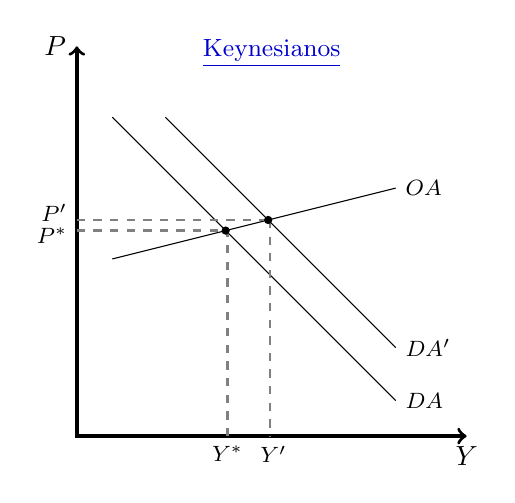
\begin{tikzpicture}[scale=0.45]
    \draw[very thick,<->] (0,11) node[left]{$P$}--(0,0)--(11,0) node[below]{$Y$};
    \draw[thin](1,5)--(9,7) node [right] {\footnotesize $OA$};
    \draw[thin](1,9)--(9,1) node [right] {\footnotesize $DA$};
    \draw[thin](2.5,9)--(9,2.5) node [right] {\footnotesize $DA'$};
    \draw[thick,gray,dashed](0, 5.8)--(4.25, 5.8);
    \draw[thick,gray,dashed](4.25, 0)--(4.25, 5.8);
    \draw[thick,gray,dashed](0, 6.1)--(5.45, 6.1);
    \draw[thick,gray,dashed](5.45, 6.1)--(5.45, 0);
    \node[left] at (0,5.65) {\footnotesize $P^{*}$};
    \node[left] at (0,6.3) {\footnotesize $P'$};
    \node[below] at (4.25,0) {\footnotesize $Y^{*}$};
    \node[below] at (5.55,0) {\footnotesize $Y'$};
    \draw[fill](4.2,5.8) circle [radius =0.1];
    \draw[fill](5.4,6.1) circle [radius =0.1];
    \node[] at(5.5,10.8) {\textcolor{blue!80!black}{\small \underline{Keynesianos}}};
    \end{tikzpicture}
    \end{center}
    \vspace{-2mm}
    \begin{itemize}
    \small
        \item Un aumento de la $DA$ logra expandir el nivel de producción (con una leve subida de $P$)
    \end{itemize}
    \end{columns}
\end{frame}


\begin{frame}{Shocks a la Oferta Agregada}

Los shocks de oferta negativos  producen un fenómeno que se conoce como \textbf{estanflación} (cae el nivel de producto y aumenta el nivel de precios)

\begin{columns}
  \column{0.5\textwidth} 
    \begin{center}
    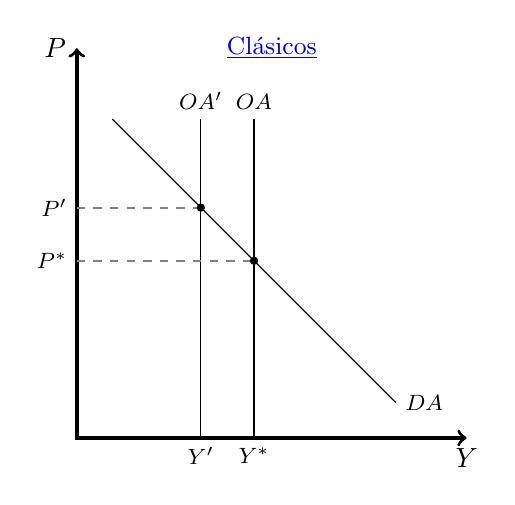
\begin{tikzpicture}[scale=0.45]
    \draw[very thick,<->] (0,11) node[left]{$P$}--(0,0)--(11,0) node[below]{$Y$};
    \draw[thin](5,0)--(5,9) node [above] {\footnotesize $OA$};
    \draw[thin](1,9)--(9,1) node [right] {\footnotesize $DA$};
    \draw[thin](3.5,0)--(3.5,9) node [above] {\footnotesize $OA'$};
    \draw[thick,gray,dashed](0, 5)--(5, 5);
    \draw[thick,gray,dashed](0, 6.5)--(3.5, 6.5);
    \node[left] at (0,5) {\footnotesize $P^*$};
    \node[left] at (0,6.5) {\footnotesize $P'$};
    \node[below] at (5,0) {\footnotesize $Y^{*}$};
    \node[below] at (3.5,0) {\footnotesize $Y'$};
    \draw[fill](3.5,6.5) circle [radius =0.1];
    \draw[fill](5,5) circle [radius =0.1];
    \node[] at(5.5,11) {\textcolor{blue!80!black}{\small \underline{Clásicos}}};
    \end{tikzpicture}
    \end{center}

\column{0.5\textwidth} 
    \begin{center}
    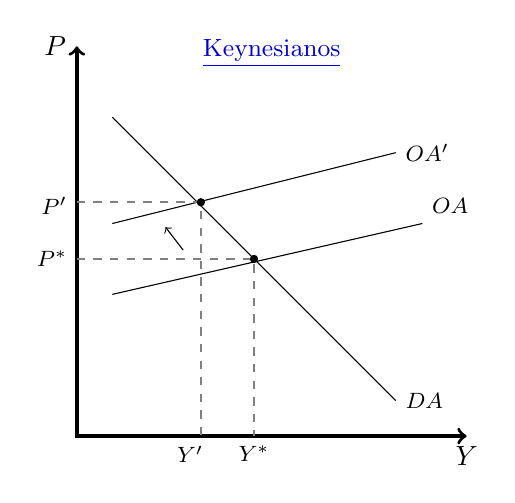
\begin{tikzpicture}[scale=0.45]
    \draw[very thick,<->] (0,11) node[left]{$P$}--(0,0)--(11,0) node[below]{$Y$};
    \draw[thin](1,6)--(9,8) node [right] {\footnotesize $OA'$};
    \draw[thin](1,4)--(9.75,6) node [above right] {\footnotesize $OA$};
    \draw[thin](1,9)--(9,1) node [right] {\footnotesize $DA$};
    \draw[thin, ->] (3,5.25)--(2.5,5.9);
    \draw[thick,gray,dashed](0, 6.6)--(3.5, 6.6)--(3.5, 0);
    \draw[thick,gray,dashed](0, 5)--(5,5)--(5, 0);
    \node[left] at (0,5) {\footnotesize $P^*$};
    \node[left] at (0,6.5) {\footnotesize $P'$};
    \node[below] at (5,0) {\footnotesize $Y^{*}$};
    \node[below] at (3.2,0) {\footnotesize $Y'$};
    \draw[fill](3.5,6.6) circle [radius =0.1];
    \draw[fill](5,5) circle [radius =0.1];
    \node[] at(5.5,10.8) {\textcolor{blue!80!black}{\small \underline{Keynesianos}}};
    \end{tikzpicture}
    \end{center}
    \end{columns}
\end{frame}

\begin{frame}{Shock Covid}
\vspace{2mm}
Los shocks a la $OA$ y $DA$ generaron una \textbf{recesión} bastante fuerte (cayó el producto de $Y^{*}$ a $Y'$), con un efecto (menos fuerte) en la inflación (los precios aumentaron de $P^*$ a $P'$). 
\begin{center}
    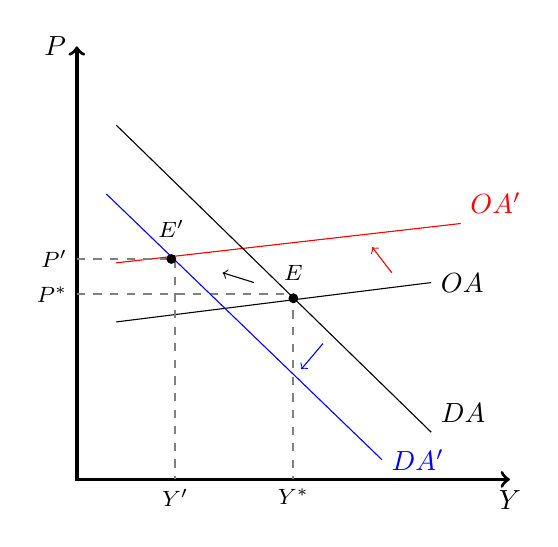
\begin{tikzpicture}[scale=0.5]
    \draw[very thick,<->] (0,11) node[left]{$P$}--(0,0)--(11,0) node[below]{$Y$};
    \draw[thin](1,4)--(9,5) node [right] {$OA$};
    \draw[thin, red](1,5.5)--(9.75,6.5) node [above right] {$OA'$};
    \draw[thick,gray,dashed](0, 5.6)--(2.5, 5.6)--(2.5, 0);
    \draw[thick,gray,dashed](0, 4.7)--(5.5,4.7)--(5.5, 0);
    \draw[thin](1,9)--(9,1.2) node [above right] {$DA$};
    \draw[thin, blue](0.75,7.25)--(7.75,0.5) node [right] {$DA'$};
    \draw[fill] (2.4,5.6) circle [radius =0.11];
    \node [above] at (2.4,5.9) {\footnotesize $E'$};
    \draw[fill] (5.5,4.6) circle [radius =0.11] ;
    \node [above] at (5.5,4.8){\footnotesize $E$};
    \draw[thin, red, ->] (8,5.25)--(7.5,5.9);
    \draw[thin, blue, ->] (6.25,3.45)--(5.7,2.8);
    \draw[thin, <-] (3.7,5.25)--(4.5,5); 
    \node[left] at (0,4.7) {\footnotesize $P^*$};
    \node[left] at (0,5.6) {\footnotesize $P'$};
    \node[below] at (5.5,0) {\footnotesize $Y^{*}$};
    \node[below] at (2.5,0) {\footnotesize $Y'$};
    \end{tikzpicture}
\end{center}
\end{frame}



\begin{frame}{Ciclos: los Clásicos}

La explicación clásica de las fluctuaciones viene por \textbf{cambios en la oferta agregada}


\vspace{2mm}
 
\begin{center}
\begin{figure}[H]
\renewcommand{\figurename}{Figure}
\begin{center}
    \begin{minipage}[b]{0.45\textwidth}
    \begin{center}
    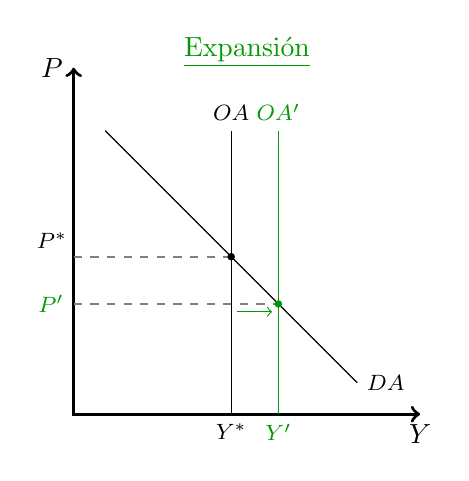
\begin{tikzpicture}[scale=0.4]
    \draw[very thick,<->] (0,11) node[left]{$P$}--(0,0)--(11,0) node[below]{$Y$};
    \draw[thin, green!60!black](6.5,0)--(6.5,9) node [above] {\footnotesize $OA'$};
    \draw[thin](5,0)--(5,9) node [above] {\footnotesize $OA$};
    \draw[thin](1,9)--(9,1) node [right] {\footnotesize $DA$};
    \draw[thin, ->, green!60!black] (5.2,3.25)--(6.3,3.25);
    \node[below] at (5,0) {\footnotesize $Y^{*}$};
    \node[below, green!60!black] at (6.5,0) {\footnotesize $Y'$};
    \node[left, green!60!black] at (0,3.5) {\footnotesize $P'$};
    \node[left] at (0.1,5.5) {\footnotesize $P^{*}$};
    \draw[thick,gray,dashed](0, 5)--(5, 5);
    \draw[thick,gray,dashed](0, 3.5)--(6.5, 3.5);
    \draw[fill](5,5) circle [radius =0.1];
    \draw[fill, green!60!black](6.5,3.5) circle [radius =0.1];
    \node[] at(5.5,11.5) {\textcolor{green!60!black}{\underline{Expansión}}};
    \end{tikzpicture}
    \end{center}
     \end{minipage}
  %  \hfill
    \begin{minipage}[b]{0.45\textwidth}
    \begin{center}
    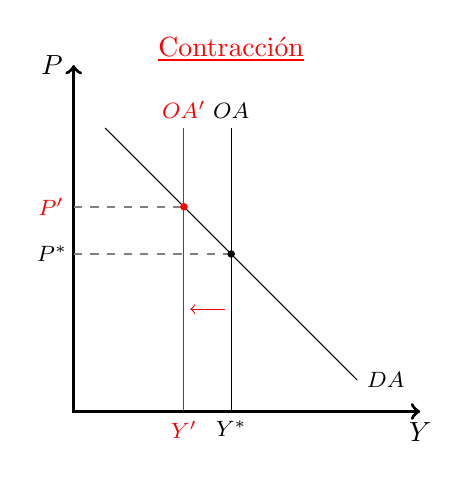
\begin{tikzpicture}[scale=0.4]
    \draw[very thick,<->] (0,11) node[left]{$P$}--(0,0)--(11,0) node[below]{$Y$};
    \draw[thin](5,0)--(5,9) node [above] {\footnotesize $OA$};
    \draw[thin, red](3.5,0)--(3.5,9) node [above] {\footnotesize $OA'$};
    \draw[thin](1,9)--(9,1) node [right] {\footnotesize $DA$};
    \draw[thin, ->, red] (4.8,3.25)--(3.7,3.25);
    \node[below] at (5,0) {\footnotesize $Y^{*}$};
    \node[below, red] at (3.5,0) {\footnotesize $Y'$};
    \node[left, red] at (0,6.5) {\footnotesize $P'$};
    \node[left] at (0.1,5) {\footnotesize $P^{*}$};
    \draw[thick,gray,dashed](0, 5)--(5, 5);
    \draw[thick,gray,dashed](0, 6.5)--(3.5, 6.5);
    \draw[fill](5,5) circle [radius =0.1];
    \draw[fill, red](3.5,6.5) circle [radius =0.1];
    \node[] at(5,11.5) {\textcolor{red}{\underline{Contracción}}};
    \end{tikzpicture}
    \end{center}
    \end{minipage}
\end{center}
\end{figure}
\end{center} 
\end{frame}

\begin{frame}{Ciclos: los Keynesianos}

La explicación keynesiana de las fluctuaciones viene por \textbf{cambios en la demanda agregada}


\vspace{2mm}

\begin{center}
\begin{figure}[H]
\renewcommand{\figurename}{Figure}
\begin{center}
    \begin{minipage}[b]{0.45\textwidth}
    \begin{center}
    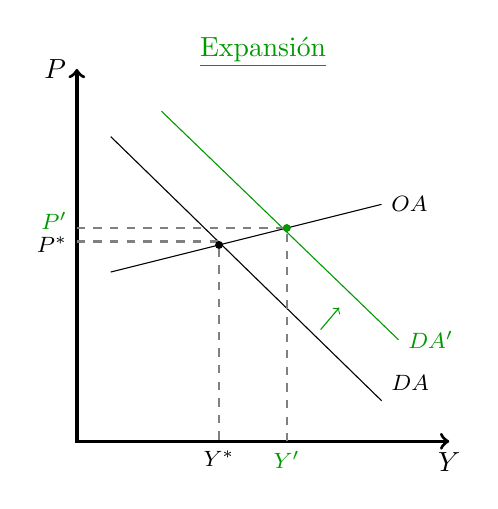
\begin{tikzpicture}[scale=0.43]
    \draw[very thick,<->] (0,11) node[left]{$P$}--(0,0)--(11,0) node[below]{$Y$};
    \draw[thin](1,5)--(9,7) node [right] {\footnotesize $OA$};
    \draw[thin](1,9)--(9,1.2) node [above right] {\footnotesize $DA$};
    \draw[thin, green!60!black](2.5,9.75)--(9.5,3) node [right] {\footnotesize $DA'$};
    \draw[thin, <-, green!60!black] (7.75,3.95)--(7.2,3.3);
    \draw[thick,gray,dashed](0, 6.3)--(6.2, 6.3)--(6.2, 0);
    \draw[thick,gray,dashed](0,5.9)--(4.2,5.9)--(4.2, 0);
    \node[left] at (0,5.8) {\footnotesize $P^{*}$};
    \node[left, green!60!black] at (0,6.5) {\footnotesize $P'$};
    \node[below,  green!60!black] at (6.2,0) {\footnotesize $Y'$};
    \node[below] at (4.2,0) {\footnotesize $Y^{*}$};
    \draw[fill, green!60!black](6.2,6.3) circle [radius =0.1];
    \draw[fill](4.2,5.8) circle [radius =0.1];
    \node[] at(5.5,11.5) {\textcolor{green!60!black}{\underline{Expansión}}};
    \end{tikzpicture}
    \end{center}
     \end{minipage}
   \hfill
    \begin{minipage}[b]{0.45\textwidth}
    \begin{center}
    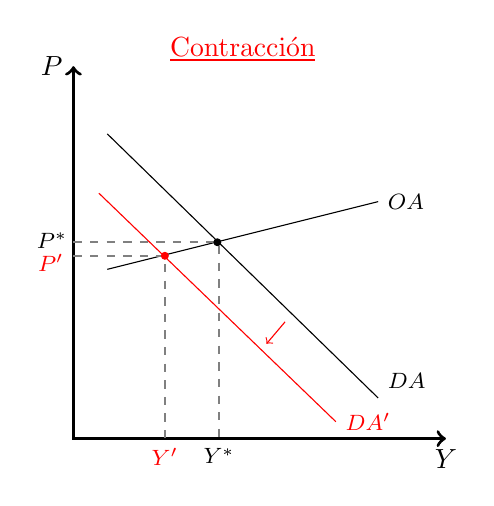
\begin{tikzpicture}[scale=0.43]
    \draw[very thick,<->] (0,11) node[left]{$P$}--(0,0)--(11,0) node[below]{$Y$};
    \draw[thin](1,5)--(9,7) node [right] {\footnotesize $OA$};
    \draw[thin](1,9)--(9,1.2) node [above right] {\footnotesize $DA$};
    \draw[thin, red](0.75,7.25)--(7.75,0.5) node [right] {\footnotesize $DA'$};
    \draw[thin, ->, red] (6.25,3.45)--(5.7,2.8);
    \draw[thick,gray,dashed](0, 5.4)--(2.7,5.4)--(2.7, 0);
    \draw[thick,gray,dashed](0,5.8)--(4.3,5.8)--(4.3, 0);
    \node[left, red] at (0,5.2) {\footnotesize $P'$};
    \node[left] at (0.1,5.85) {\footnotesize $P^{*}$};
    \node[below] at (4.3,0) {\footnotesize $Y^{*}$};
    \node[below, red] at (2.7,0) {\footnotesize $Y'$};
    \draw[fill, red](2.7,5.4) circle [radius =0.1];
    \draw[fill](4.25,5.8) circle [radius =0.1];
    \node[] at(5,11.5) {\textcolor{red}{\underline{Contracción}}};
    \end{tikzpicture}
    \end{center}
    \end{minipage}
\end{center}
\end{figure}
\end{center} 
\end{frame}

\begin{frame}{¿Por qué usar el enfoque Keynesiano en el corto plazo?}
    \begin{itemize}
        \item \textbf{Supuesto principal:} Rigidez de precios y salarios en el corto plazo.
        \item \textbf{Determina:}
        \begin{itemize}
            \item La demanda agregada define el nivel de producción.
            \item Desempleo y recursos ociosos pueden existir.
        \end{itemize}
        \item En el corto plazo, el enfoque Keynesiano es útil para gestionar fluctuaciones económicas y combatir el desempleo.
        \item En contextos donde los precios y salarios son flexibles, el enfoque clásico puede ser más adecuado.
        \item \textbf{Implicaciones prácticas:}
        \begin{itemize}
            \item Políticas fiscales expansivas o monetarias expansivas pueden ser efectivas.
            \item Permite intervenir durante recesiones para estimular la economía.
        \end{itemize}
    \end{itemize}
\end{frame}

\begin{frame}{¿Por qué usar el enfoque Clásico en el largo plazo?}
    \begin{itemize}
        \item \textbf{Supuesto principal:} Flexibilidad total de precios y salarios.
        \item \textbf{Determina:}
        \begin{itemize}
            \item El producto depende de la capacidad productiva (siempre hay pleno empleo).
            \item Los ajustes ocurren naturalmente, principalmente, por cambios en la productividad.
        \end{itemize}
        \item En el largo plazo, el enfoque clásico es preferible porque garantiza un equilibrio natural y sostenible.
        \item \textbf{Implicaciones prácticas:}
        \begin{itemize}
            \item Las intervenciones expansivas solo generan inflación sin aumentar el producto.
            \item Las políticas deben centrarse en mejorar capital físico, capital humano y tecnología.
        \end{itemize}
    \end{itemize}
\end{frame}

% \begin{frame}{Esta sería la secuencia de causalidad}

% \centering\includegraphics[width=11cm]{../Figures/P18.png}\

% \end{frame}

\end{document}